\documentclass[11pt,a4paper,openany]{report}
\usepackage[T1]{fontenc}
\usepackage[utf8]{inputenc}
\usepackage{lmodern}
\usepackage{microtype}
\usepackage{amsmath,amssymb,mathtools,bm}
\usepackage{booktabs,array,longtable,tabularx}
\usepackage{xcolor}
\usepackage[margin=22mm,headheight=23pt]{geometry}
\usepackage{enumitem}
\usepackage{fancyhdr}
\usepackage{fancyvrb}
\usepackage{graphicx}
\usepackage{url}
\usepackage{xurl}
\usepackage{hyperref}
\definecolor{finblue}{HTML}{1F5A99}
\definecolor{fingreen}{HTML}{19733A}
\definecolor{finorange}{HTML}{D55E00}
\definecolor{finred}{HTML}{A61B1B}
\definecolor{finviolet}{HTML}{6A3D9A}
\definecolor{fingray}{HTML}{4D4D4D}
\hypersetup{
  unicode=true,
  colorlinks=true,
  linkcolor=finblue,
  citecolor=fingreen,
  urlcolor=finblue,
  pdftitle={Atlas Drugiej Generacji: Pochodne Obiekty Nadsolitona},
  pdfauthor={Krzysztof Żuchowski},
  pdfsubject={Systematyczne przeszukanie kombinacji FIN C01-C12, obiekty O01-O15 i synteza G01-G10},
  pdfkeywords={FIN, nadsoliton, Stieltjes functions, Schur complement, memory kernel, operator theory, information geometry}
}
\pagestyle{fancy}
\fancyhf{}
\fancyhead[L]{\small Atlas Drugiej Generacji}
\fancyhead[R]{\small Release 10.23}
\fancyfoot[C]{\thepage}
\setlength{\parindent}{0pt}
\setlength{\parskip}{0.55em}
\setlist{nosep,leftmargin=2em}
\setcounter{tocdepth}{2}
\setcounter{secnumdepth}{3}
\emergencystretch=3em
\newcommand{\one}{\bm 1}
\newcommand{\C}{\mathbb C}
\newcommand{\R}{\mathbb R}
\newcommand{\Z}{\mathbb Z}
\newcommand{\statusProven}{\textcolor{fingreen}{[Proven]}}
\newcommand{\statusStrong}{\textcolor{finblue}{[Strong evidence]}}
\newcommand{\statusModerate}{\textcolor{finviolet}{[Moderate evidence]}}
\newcommand{\statusWeak}{\textcolor{fingray}{[Weak evidence]}}
\newcommand{\statusSpeculative}{\textcolor{finorange}{[Speculative]}}
\newcommand{\statusRefuted}{\textcolor{finred}{[Refuted]}}
\begin{document}
\hypersetup{pageanchor=false}
\begin{titlepage}
\centering
\vspace*{12mm}
{\Large\bfseries FIN --- Release 10.23\par}
\vspace{12mm}
{\Huge\bfseries Atlas Drugiej Generacji\par}
\vspace{5mm}
{\LARGE\bfseries Pochodne Obiekty Nadsolitona\par}
\vspace{8mm}
{\Large Systematyczne przeszukanie C01...C12,\\
konstrukcja O01...O15 i synteza G01...G10\par}
\vspace{18mm}
{\Large Krzysztof \.Zuchowski\par}
\vspace{2mm}
{\normalsize Independent Researcher --- Fractal Information Theory Project\par}
\vspace{2mm}
{\normalsize ORCID: \href{https://orcid.org/0009-0002-0909-3613}{0009-0002-0909-3613}\par}
\vspace{10mm}
{\large 28 lipca 2026\par}
\vfill
\begin{minipage}{0.9\textwidth}
\small
\textbf{Główny obiekt.}
\[
E\longmapsto \operatorname{Schur}_{V\setminus E}(zI+A),\qquad
\Sigma_E(z)=A_{EH}(zI+A_{HH})^{-1}A_{HE}.
\]
Kontekstowe redukcje składają się, a samoenergie są dodatnimi operatorowymi
funkcjami Stieltjesa generującymi dokładną pamięć.

\medskip
\textbf{Granica.} Raport nie eksportuje selektora, skali fizycznej,
mostu legacy--strict, role transfer ani walidacji laboratoryjnej.

\medskip
\textbf{Repozytorium.}
\url{https://github.com/hyconiek/Fractal-Nadsoliton-Theory}

\textbf{Licencja.} CC BY 4.0.
\end{minipage}
\vfill
\end{titlepage}
\hypersetup{pageanchor=true}
\pagenumbering{roman}
\tableofcontents
\clearpage
\pagenumbering{arabic}

\chapter*{Confidence convention}
\addcontentsline{toc}{chapter}{Confidence convention}

\begin{itemize}
\item 
\textbf{\statusProven{}} --- rezultat analityczny albo jawna to\.zsamość numeryczna z tolerancją.

\item 
\textbf{\statusStrong{}} --- stabilna konstrukcja z niezamkniętym twierdzeniem ogólnym lub interpretacją.

\item 
\textbf{\statusModerate{}} --- typowany mechanizm, którego identyfikowalność albo unikalność pozostaje otwarta.

\item 
\textbf{\statusSpeculative{}} --- hipoteza konstrukcyjna przeznaczona do falsyfikacji.

\item 
\textbf{\statusRefuted{}} --- połączenie odrzucone w zadanej klasie, zwykle z powodu braku wspólnej operacji.

\end{itemize}

\chapter{1. Streszczenie wykonawcze}

Druga faza atlasu nie pyta ju\.z tylko, do czego podobne są puzzle C01...C12. Pyta:

\[
\text{jakie nowe obiekty mo\.zna skonstruować, gdy ich operacje są składane?}
\]

Wykonano skończone, reprodukowalne przeszukanie:

\begin{center}
\begingroup\small
\setlength{\tabcolsep}{2.5pt}
\renewcommand{\arraystretch}{1.16}
\begin{longtable}{@{}p{0.420\textwidth}p{0.420\textwidth}@{}}
\toprule
\textbf{Klasa} & \textbf{Liczba} \\
\midrule
\endhead
pojedyncze puzzle & 12 \\
wszystkie pary & 66 \\
wszystkie trójki & 220 \\
wybrane sprzę\.zenia 4--6 puzzli & 7 \\
razem przeskanowanych kombinacji & 305 \\
wiersze z typowanym obiektem lub mechanizmem & 109 \\
odrzucone czysto wizualne zestawienia & 184 \\
obiekty drugiej generacji O & 15 \\
obiekty trzeciej generacji G & 10 \\
\bottomrule
\end{longtable}
\endgroup
\end{center}

\begin{figure}[htbp]
\centering
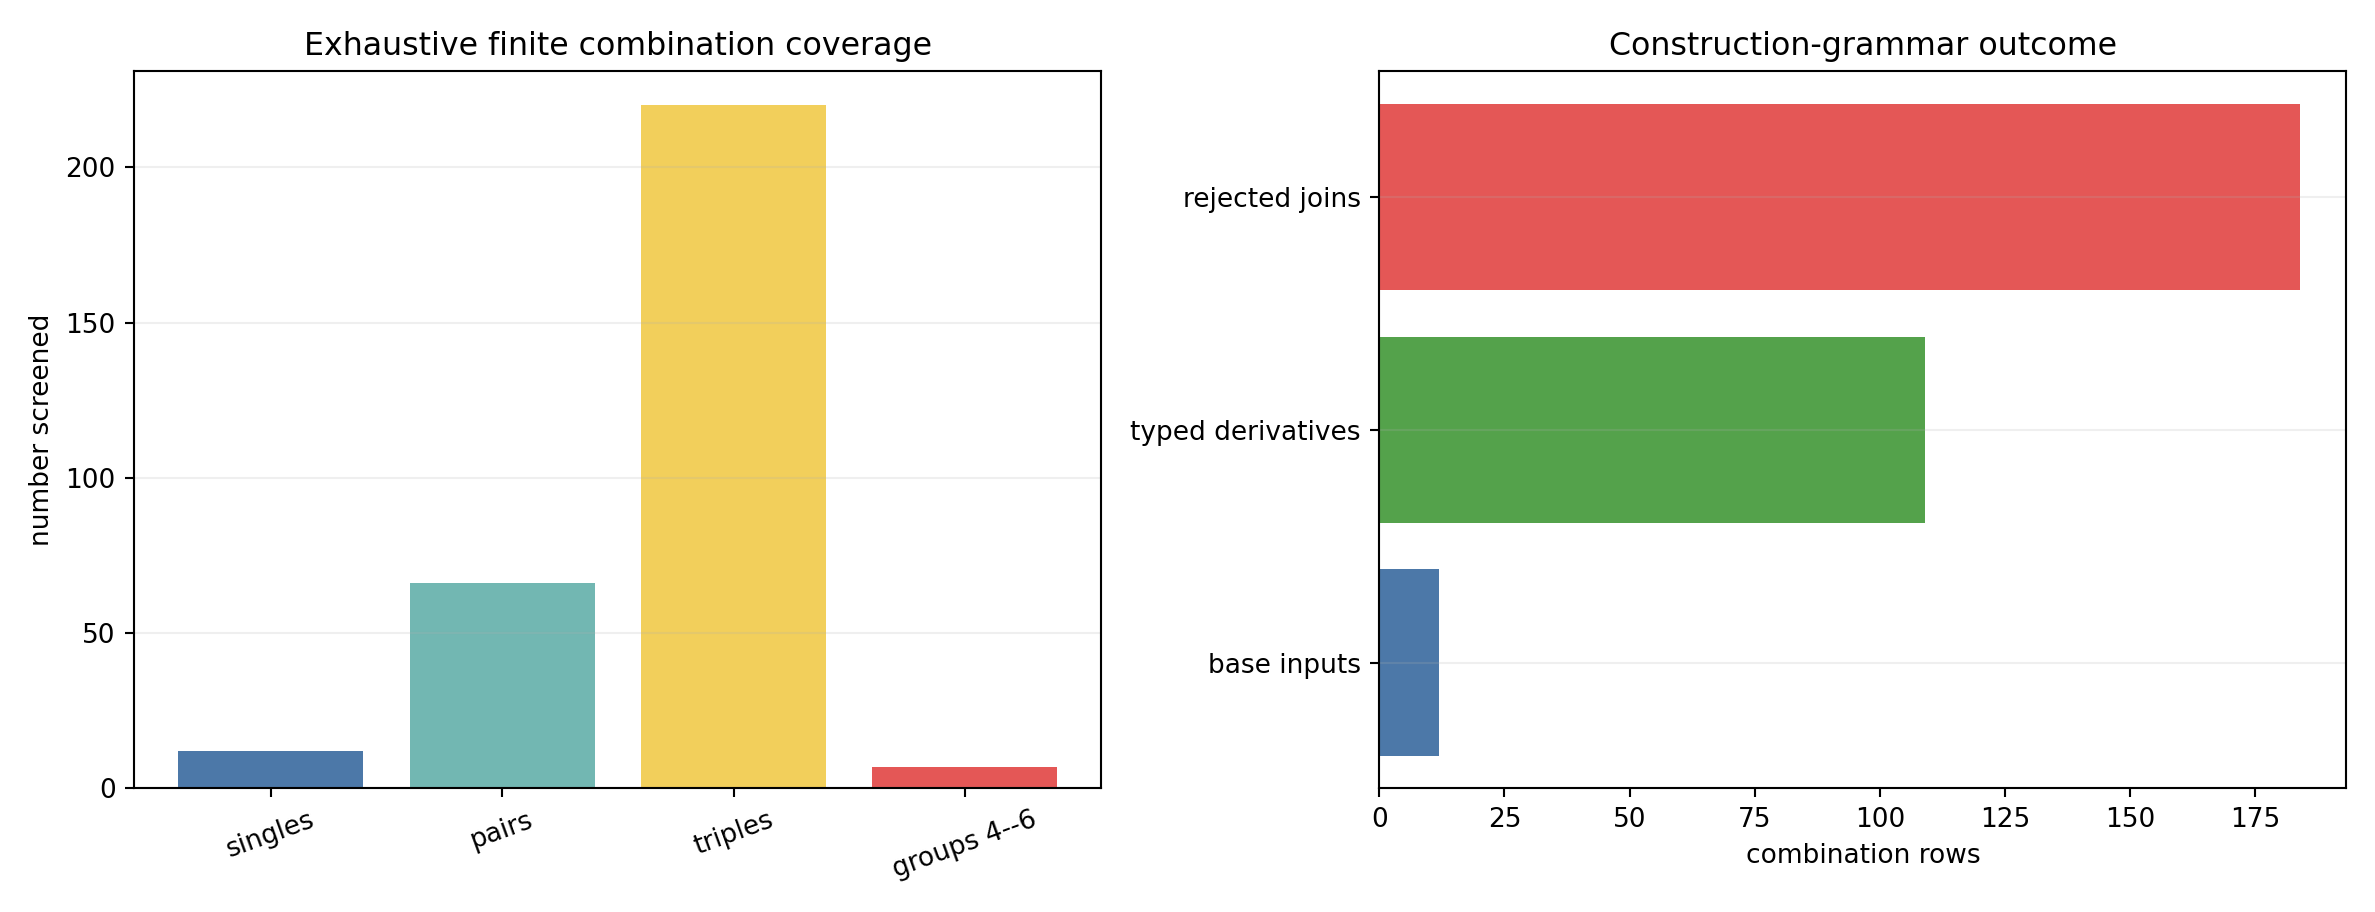
\includegraphics[width=0.97\textwidth]{FIN_Second_Generation_Atlas_Figures/combination_search_coverage.png}
\caption{Pełne pokrycie singli, par i trójek oraz wynik jawnej gramatyki konstrukcji.}
\end{figure}

Najmocniejszym odkrytym obiektem nie jest pojedyncza macierz, lecz kontekstowa rodzina:

\[
\mathfrak S_A:
E\longmapsto
B_E(z)
=\operatorname{Schur}_{V\setminus E}(zI+A),
\qquad z>0.
\]

Dla ka\.zdego obserwowanego kontekstu \(E\), ukryty sektor generuje samoenergię:

\[
\Sigma_E(z)
=A_{EH}(zI+A_{HH})^{-1}A_{HE}.
\]

Rodzina ma trzy ścisłe własności:

\begin{enumerate}
\item 
redukcje zagnie\.zd\.zone składają się dokładnie dzięki łączności dopełnienia Schura;

\item 
\(\Sigma_E(z)\) jest dodatnią operatorową funkcją Stieltjesa;

\item 
odwrotna transformata Laplace'a jest jądrem pamięci zredukowanego procesu.

\end{enumerate}

Obiekt generacji G02 nazywamy:

\begin{quote}\itshape
\textbf{Stieltjes--Schur Context Functor} --- kontekstowym funktorem Stieltjesa--Schura.

\end{quote}

\statusProven{} jako skończona algebra operatorowa.\\
\statusSpeculative{} jako fundament fizycznej ontologii.

Drugim szczególnie obiecującym obiektem jest chiralna podatność pamięci:

\[
\Xi_E(z)
=
\left.
\partial_\theta\Sigma_E(z,\theta)
\right|_{\theta=0},
\]

która jest niezerowa i nieparzysta pod odbiciem, ale pozostaje \textbf{odbiornikiem} wło\.zonego skrętu \(\theta\), nie źródłem orientacji. \statusStrong{}

Trzeci wynik porządkuje "ujemne sprzę\.zenie informacji". Zanik dostępnej informacji mo\.ze być opisany bez modyfikowania jądra przez ledger kontrakcji:

\[
\mathcal L_t(p,q)
=D(p\Vert q)-D(P_tp\Vert P_tq)\geq0.
\]

To utrata rozró\.znialności w dostępnym kanale. Nie jest to automatycznie zniszczenie informacji ani energia termodynamiczna. \statusProven{}

\chapter{2. Metoda generowania, a nie dopasowywania}

Ka\.zda kombinacja przechodzi pięć bramek:

\begin{enumerate}
\item 
\textbf{Operacja wspólna:} czy działania puzzli mo\.zna zło\.zyć z poprawnymi typami wejścia i wyjścia?

\item 
\textbf{Nowy obiekt:} czy wynik jest czymś więcej ni\.z listą składników?

\item 
\textbf{Nowa przestrzeń:} czy obiekt \.zyje w rozpoznawalnej przestrzeni operatorów, funkcjonałów, miar albo funktorów?

\item 
\textbf{Obserwabla i dynamika:} czy konstrukcja daje liczbę, rekord albo ewolucję podlegającą testowi?

\item 
\textbf{Falsification gate:} jaki wynik obali tę konstrukcję lub jej silniejszą interpretację?

\end{enumerate}

Zasada stop:

\begin{quote}\itshape
Jeśli kombinacja nie ma typowanej operacji, nie generuje obiektu. Podobieństwo słowne lub wizualne zostaje oznaczone jako \statusRefuted{}.

\end{quote}

Pełny wynik dla wszystkich 305 kombinacji znajduje się w:

FIN\_Second\_Generation\_Combination\_Search.csv.

Ka\.zdy wiersz zawiera:

\begin{itemize}
\item 
operację wspólną;

\item 
kandydat obiektu;

\item 
przestrzeń obiektów;

\item 
nową obserwablę;

\item 
nową dynamikę;

\item 
status;

\item 
informację, czy wynik jest nowym sprzę\.zeniem, czy tylko dziedziczy obiekt ni\.zszego rzędu.

\end{itemize}

\chapter{3. Inwentarz bazowy C01...C12}

\begin{center}
\begingroup\small
\setlength{\tabcolsep}{2.5pt}
\renewcommand{\arraystretch}{1.16}
\begin{longtable}{@{}p{0.055\textwidth}p{0.190\textwidth}p{0.420\textwidth}p{0.195\textwidth}@{}}
\toprule
\textbf{ID} & \textbf{Obiekt bazowy} & \textbf{Operacja dominująca} & \textbf{Ograniczenie krytyczne} \\
\midrule
\endhead
C01 & strict kernel & splot/\allowbreak{}spektralizacja na \(Z_{12}\) & brak automatycznego kontinuum \\
C02 & legacy intermediate bridge & profil propagatorowo-tłumiący & brak pełnej mapy completion i role transfer \\
C03 & \(A=sI-W\succeq0\) & forma Dirichleta i rachunek widmowy & brak jednostki energii \\
C04 & \(e^{-itA},e^{-tA}\) & dwa promienie rachunku funkcyjnego & ró\.zne semantyki operacyjne \\
C05 & Green/\allowbreak{}resolwent/\allowbreak{}działanie & odwracanie operatora i wariacja & propagator nie wyznacza pełnej interakcji \\
C06 & cocykl/\allowbreak{}chiralne odbiorniki & znak pod inwersją & brak niepremisowego znaku \\
C07 & fraktalna kompresja Schura & eliminacja stopni swobody & strict nie jest statycznym fixed pointem \\
C08 & adaptacja i pamięć & sprzę\.zenie zwrotne operator--rekord & prawo uczenia jest dodatkowe \\
C09 & informacja/\allowbreak{}geometria & entropia, Fisher, dyfuzja & brak jednostki fizycznej \\
C10 & proces operacyjny & przygotowanie--instrument--środowisko--rekord & konkretny lab pozostaje zewnętrzny \\
C11 & przeszkoda skali & iloraz przez \(\mathbb R_{>0}\) & brak kanonicznej sekcji \\
C12 & przeszkoda selektora & iloraz/\allowbreak{}torsor orientacji & QW-2191 pozostaje otwarte \\
\bottomrule
\end{longtable}
\endgroup
\end{center}

\chapter{4. Tabela główna: obiekty drugiej generacji}

\begin{center}
\begingroup\fontsize{7}{8.4}\selectfont
\setlength{\tabcolsep}{2.5pt}
\renewcommand{\arraystretch}{1.16}
\begin{longtable}{@{}p{0.084\textwidth}p{0.161\textwidth}p{0.272\textwidth}p{0.144\textwidth}p{0.144\textwidth}p{0.055\textwidth}@{}}
\toprule
\textbf{Kombinacja FIN} & \textbf{Powstały obiekt} & \textbf{Matematyczna postać} & \textbf{Analogiczne dziedziny} & \textbf{Nowa intuicja} & \textbf{Status} \\
\midrule
\endhead
C03+\allowbreak{}C05+\allowbreak{}C07 & O01 Dynamic Spectral Compression Kernel & \(\Sigma_E(z)=A_{EH}(zI+A_{HH})^{-1}A_{HE}\) & Feshbach, Mori--Zwanzig, Kron reduction & redukcja dynamiczna generuje pamięć & \statusProven{} \\
C03+\allowbreak{}C05+\allowbreak{}C07 & O02 Frequency-Dependent Effective Action & \(S_z[x]=\frac12\langle x,(zI+A_{EE}-\Sigma_E(z))x\rangle-\langle j,x\rangle\) & effective action, influence functional & Green, kompresja i wariacja stają się jednym obiektem & \statusProven{} \\
C05+\allowbreak{}C07+\allowbreak{}C10 & O03 Resolvent Context Presheaf & \(E\mapsto\operatorname{Schur}_{V\setminus E}(zI+A)\) & teoria kategorii, open systems, network reduction & ka\.zdy obserwator/\allowbreak{}kontekst ma zgodny operator efektywny & \statusProven{} \\
C03+\allowbreak{}C06+\allowbreak{}C12 & O04 Chiral Spectral Response Bundle & \((M_R,\Lambda,C_\chi,\operatorname{Im}B)\) & resource theory of asymmetry, harmonic analysis & ró\.zne chiralne testy są odbiornikami jednego typu zasobu & \statusStrong{} \\
C06+\allowbreak{}C07+\allowbreak{}C10 & O05 Chiral Memory Susceptibility & \(\Xi_E(z)=\partial_\theta\Sigma_E(z,\theta)|_0\) & Kubo response, flux susceptibility, open systems & ukryte stopnie swobody mają chiralną odpowiedź pamięci & \statusStrong{} \\
C03+\allowbreak{}C04+\allowbreak{}C09 & O06 Heat Information Metric Tower & \(D_t^2(x,y)=\sum_z|P_t(x,z)-P_t(y,z)|^2/\pi_z\) & diffusion maps, information geometry & geometryczna "odległość informacji" jest wieloskalowa & \statusProven{} \\
C10+\allowbreak{}C11 & O07 Operational Calibration Torsor & \((A,\tau)\sim(cA,\tau/c)\) & metrologia, gauge fixing, system identification & eksperyment wybiera skalę, algebra daje tylko orbitę & \statusProven{} \\
C01+\allowbreak{}C03+\allowbreak{}C11 & O08 Projective Spectral Fingerprint & \((\lambda_1/\lambda_{\max},\ldots)\) & inverse spectral theory, control & część predykcji jest testowalna przed kalibracją absolutną & \statusProven{} \\
C04+\allowbreak{}C09+\allowbreak{}C10 & O09 Information Contraction Ledger & \(\mathcal L_t=D(p\Vert q)-D(P_tp\Vert P_tq)\) & data processing, statistics, sensory bottlenecks & "ubytek" to utrata dostępnej rozró\.znialności & \statusProven{} \\
C04+\allowbreak{}C07+\allowbreak{}C10 & O10 Dual-Ray Reduced Process Tensor & \(\mathcal T_r[\mathcal M_1,\ldots,\mathcal M_r]\) dla projekcji wave/\allowbreak{}heat & process tensors, cybernetyka, causal models & pamięć ujawnia się dopiero przy interwencjach wieloczasowych & \statusModerate{} \\
C08+\allowbreak{}C09+\allowbreak{}C10 & O11 Adaptive Memory Geometry Flow & \((\dot A,\dot q)=(-\nabla_A\mathcal L,-\operatorname{grad}_F\mathcal L)\) & neural operators, adaptive networks, biological plasticity & uczenie mo\.ze odbywać się w przestrzeni geometrii pamięci & \statusSpeculative{} \\
C05+\allowbreak{}C07+\allowbreak{}C08 & O12 Multiscale Memory Functor & \(\Sigma^{(0)}(z)\to\Sigma^{(1)}(z)\to\cdots\) & continued fractions, hierarchical reservoirs, RG & fraktalny fixed point nale\.zy szukać w przestrzeni funkcji pamięci & \statusStrong{} \\
C01+\allowbreak{}C02+\allowbreak{}C07 & O13 Legacy-Strict Completion-Defect Tower & \(\Delta_n=K_{\rm strict}^{(n)}-\mathcal C_n[K_{\rm legacy}^{(n)}]\) & error propagation, RG defects, obstruction theory & most mo\.zna badać przez dynamikę defektu, nie deklarację podobieństwa & \statusModerate{} \\
C06+\allowbreak{}C09+\allowbreak{}C12 & O14 Spectral Asymmetry Transport Cost & \(\inf_{\Phi\ {\rm covariant}}\operatorname{Cost}(\Phi)\) & optimal transport, resource conversion & orientacja ma koszt operacyjny, ale koszt nie wybiera znaku & \statusModerate{} \\
C10+\allowbreak{}C11+\allowbreak{}C12 & O15 Two-Torsor Physicalization Bundle & \(\mathcal T_{\rm scale}\times\mathcal T_{\rm orient}\) & principal bundles, reference frames, calibration & skala i orientacja wymagają dwóch oddzielnych sekcji & \statusStrong{} \\
\bottomrule
\end{longtable}
\endgroup
\end{center}

\chapter{5. Co obiekty wyjaśniają, czego nie wyjaśniają i jak je obalić}

\begin{center}
\begingroup\small
\setlength{\tabcolsep}{2.5pt}
\renewcommand{\arraystretch}{1.16}
\begin{longtable}{@{}p{0.128\textwidth}p{0.233\textwidth}p{0.210\textwidth}p{0.290\textwidth}@{}}
\toprule
\textbf{Obiekt pochodny} & \textbf{Co wyjaśnia} & \textbf{Czego NIE wyjaśnia} & \textbf{Test falsyfikujący} \\
\midrule
\endhead
O01 DSCK & dokładną pamięć po eliminacji & fizycznego środowiska i skali & stałość \(\Sigma_E(z)\) mimo niezerowego sprzę\.zenia \\
O02 Effective Action & dokładną odpowiedź źródłową na kontekście & oddziaływań nieliniowych i kwantyzacji & niezgodność rozwiązania stacjonarnego z blokowym Greenem \\
O03 Context Presheaf & zgodność redukcji zagnie\.zd\.zonych & unikalnego wyboru kontekstu obserwatora & niezerowy residual bezpośredni--zagnie\.zd\.zony \\
O04 Chiral Bundle & wspólną kowariancję odbiorników znaku & źródła znaku & stan symetryczny dający niezerowy odbiornik odd \\
O05 Chiral Memory & odpowiedź pamięci na skręt fazowy & selektora \(\theta\) & brak nieparzystości pod odbiciem \\
O06 Metric Tower & geometrię rozró\.znialności & SI length i Lorentz signature & wzrost odległości przy kontrakcyjnej semigrupie \\
O07 Calibration Torsor & nieidentyfikowalność absolutnej skali & źródła wzorca laboratoryjnego & rozró\.znienie \((A,\tau)\) i \((cA,\tau/c)\) z tego samego \(P_\tau\) \\
O08 Fingerprint & bezskalowe przewidywania widmowe & absolutnej energii & zmiana fingerprintu pod dodatnim skalowaniem \\
O09 Information Ledger & dostępny ubytek rozró\.znialności & termodynamicznej energii i ontologicznego zniszczenia informacji & naruszenie data processing \\
O10 Process Tensor & operacyjną pamięć i rolę interwencji & konkretnej mikroskopowej dylatacji & model bez pamięci reprodukujący wszystkie interwencje \\
O11 Adaptive Flow & mo\.zliwy mechanizm uczenia operatora & strict source law i biologię & brak przewagi hold-out nad statycznym modelem \\
O12 Memory Functor & hierarchiczną kompresję dynamiczną & fixed pointu strict & brak stabilizacji jakiejkolwiek klasy funkcjonalnej \\
O13 Defect Tower & gdzie i jak nie domyka się bridge & role transfer i completion theorem & residual malejący do zera bez target coding \\
O14 Transport Cost & ilość potrzebnego zasobu asymetrii & kanonicznego wyboru zasobu & darmowa operacja zwiększająca monotone \\
O15 Two-Torsor Bundle & niezale\.zność problemu skali i orientacji & źródła obu sekcji & wewnętrzna jedna dana jednocześnie i kanonicznie zamykająca oba torsory \\
\bottomrule
\end{longtable}
\endgroup
\end{center}

\chapter{6. Ranking O01...O15}

Skale:

\begin{itemize}
\item 
nowość 0--5;

\item 
ścisłość matematyczna 0--5;

\item 
związek z FIN 0--5;

\item 
falsyfikowalność 0--5;

\item 
ryzyko nadinterpretacji 0--5, gdzie 5 oznacza ryzyko najwy\.zsze.

\end{itemize}

\begin{figure}[htbp]
\centering
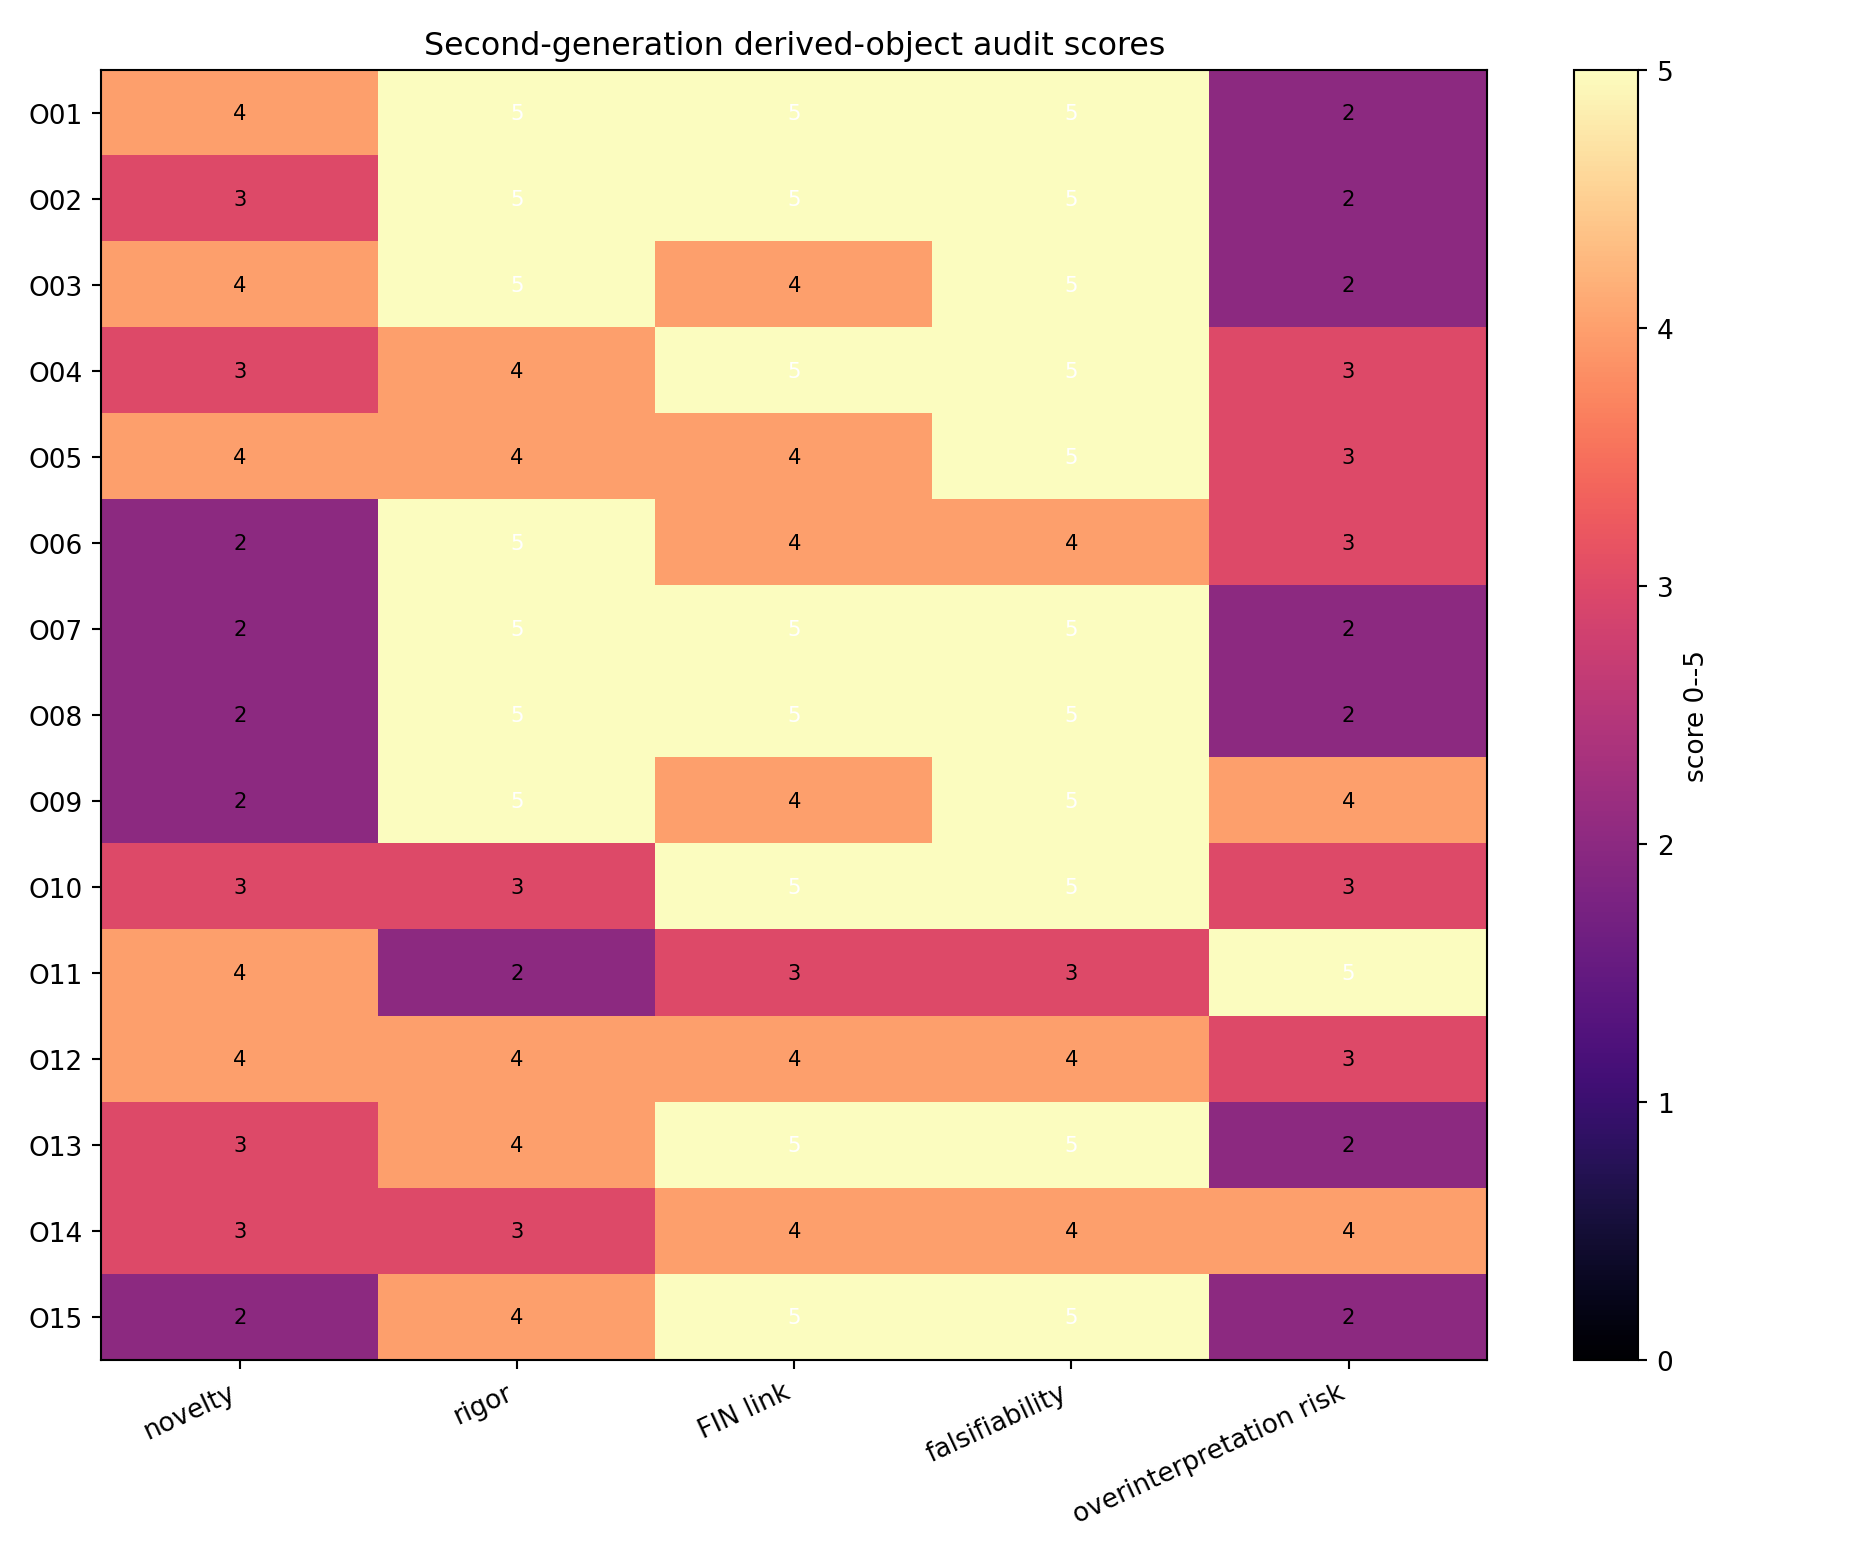
\includegraphics[width=0.97\textwidth]{FIN_Second_Generation_Atlas_Figures/derived_object_score_matrix.png}
\caption{Audyt punktowy O01--O15; ryzyko nadinterpretacji ma przeciwną semantykę do pozostałych ocen.}
\end{figure}

\begin{center}
\begingroup\fontsize{7}{8.4}\selectfont
\setlength{\tabcolsep}{2.5pt}
\renewcommand{\arraystretch}{1.16}
\begin{longtable}{@{}p{0.061\textwidth}p{0.123\textwidth}p{0.164\textwidth}p{0.061\textwidth}p{0.328\textwidth}p{0.123\textwidth}@{}}
\toprule
\textbf{ID} & \textbf{Nowość} & \textbf{Ścisłość} & \textbf{FIN} & \textbf{Falsyfikowalność} & \textbf{Ryzyko} \\
\midrule
\endhead
O01 & 4 & 5 & 5 & 5 & 2 \\
O02 & 3 & 5 & 5 & 5 & 2 \\
O03 & 4 & 5 & 4 & 5 & 2 \\
O04 & 3 & 4 & 5 & 5 & 3 \\
O05 & 4 & 4 & 4 & 5 & 3 \\
O06 & 2 & 5 & 4 & 4 & 3 \\
O07 & 2 & 5 & 5 & 5 & 2 \\
O08 & 2 & 5 & 5 & 5 & 2 \\
O09 & 2 & 5 & 4 & 5 & 4 \\
O10 & 3 & 3 & 5 & 5 & 3 \\
O11 & 4 & 2 & 3 & 3 & 5 \\
O12 & 4 & 4 & 4 & 4 & 3 \\
O13 & 3 & 4 & 5 & 5 & 2 \\
O14 & 3 & 3 & 4 & 4 & 4 \\
O15 & 2 & 4 & 5 & 5 & 2 \\
\bottomrule
\end{longtable}
\endgroup
\end{center}

Najlepszy bilans daje O01. Najbogatszą strukturę wy\.zszego rzędu daje połączenie O01+O03+O12. Największe ryzyko nadinterpretacji ma O11, poniewa\.z analogie do uczenia i biologii nie są prawem źródłowym FIN.

\chapter{7. Twierdzenia wygenerowane w drugiej fazie}

\section{7.1. O01 nale\.zy do operatorowej klasy Stieltjesa}

Dla \(z>0\), \(A_{HH}\succeq0\):

\[
\Sigma_E(z)
=A_{EH}(zI+A_{HH})^{-1}A_{HE}.
\]

Dla ka\.zdego \(n\geq0\):

\[
(-1)^n\Sigma_E^{(n)}(z)
=n!\,
A_{EH}(zI+A_{HH})^{-(n+1)}A_{HE}
\succeq0.
\]

Zatem \(\Sigma_E\) jest całkowicie monotoniczną dodatnią funkcją operatorową. \statusProven{}

Znaczenie:

\begin{itemize}
\item 
jej bieguny i miara spektralna kodują ukryte mody;

\item 
jej odwrotna transformata Laplace'a jest zanikającym jądrem pamięci;

\item 
przestrzeń właściwych kandydatów dla dynamicznej kompresji jest znacznie wę\.zsza ni\.z "wszystkie funkcje macierzowe".

\end{itemize}

Test numeryczny strict \(Z_{12}\) dla rzędów \(0,\ldots,4\) daje minimalne wartości własne większe od \(-6.4\times10^{-17}\), czyli dodatniość do błędu zmiennoprzecinkowego.

\section{7.2. O03 składa się funktorialnie}

Niech \(G\subset F\subset E\subset V\). Dla \(B(z)=zI+A\):

\[
\operatorname{Schur}_{E\setminus G}
\left(
\operatorname{Schur}_{V\setminus E}B
\right)
=
\operatorname{Schur}_{V\setminus G}B.
\]

Po właściwym rozpisaniu kroków pośrednich jest to łączność eliminacji Gaussa/\allowbreak{}dopełnienia Schura. \statusProven{}

Dla wybranych kontekstów strict \(Z_{12}\) residual bezpośrednia--zagnie\.zd\.zona redukcja wynosi:

\[
2.47\times10^{-16}.
\]

To uzasadnia słowo "funktor" w ograniczonym sensie: poset kontekstów i morfizmy redukcji tworzą zgodny diagram operatorów. Nie udowodniono aksjomatów snopa ani kontekstualności kwantowej.

\section{7.3. O02 rekonstruuje dokładny Green kontekstu}

Niech:

\[
B_E(z)=zI+A_{EE}-\Sigma_E(z).
\]

Funkcjonał:

\[
S_z[x;j]
=\frac12\langle x,B_E(z)x\rangle-\langle j,x\rangle
\]

ma stacjonarne rozwiązanie:

\[
x_\star=B_E(z)^{-1}j
=
\left[(zI+A)^{-1}\right]_{EE}j.
\]

Residual stacjonarności w audycie:

\[
4.90\times10^{-16}.
\]

\statusProven{}

Jest to ścisła rekonstrukcja działania efektywnego z resolwentu. Nie jest pełnym działaniem fizycznym, poniewa\.z \(z\), jednostka działania, miara i interakcje pozostają dodatkowymi danymi.

\section{7.4. O05: pamięć posiada chiralny kierunek odpowiedzi}

Wprowadź hermitowską rodzinę skręconych operatorów \(A(\theta)\), gdzie skok o \(d\) otrzymuje fazę \(e^{id\theta}\). Następnie:

\[
\Xi_E(z)
=
\left.\partial_\theta
\left[
A_{EH}(\theta)
(zI+A_{HH}(\theta))^{-1}
A_{HE}(\theta)
\right]\right|_{\theta=0}.
\]

Dla podziału even/\allowbreak{}odd strict \(Z_{12}\):

\[
\|\Xi_E(0.2)\|_2=1.2175076427.
\]

Dla odbicia \(R\):

\[
R_E\Xi_E(z)R_E=-\Xi_E(z),
\]

z residualem:

\[
2.17\times10^{-16}.
\]

\statusProven{} dla zadanej rodziny skrętu i podziału.

Jednocześnie:

\[
C_\chi
=
\left.
\frac{d}{d\theta}\operatorname{Tr}[\rho A(\theta)]
\right|_{\theta=0},
\]

z residualem \(3.23\times10^{-13}\). To podnosi \(C_\chi\) z ad hoc wskaźnika do jawnej odpowiedzi na flux twist. \statusProven{}

Wa\.zne: \(\theta\) i jego znak są wprowadzone w rodzinie testowej. O05 nie rozładowuje QW-2191.

\section{7.5. O09: ujemne sprzę\.zenie informacyjne jako kontrakcja kanału}

Dla kanału Markowa \(P_t\) i dodatnich rozkładów \(p,q\):

\[
D(P_tp\Vert P_tq)\leq D(p\Vert q).
\]

Definiujemy:

\[
\mathcal L_t(p,q)
=D(p\Vert q)-D(P_tp\Vert P_tq)\geq0.
\]

W 1000 deterministycznie odtwarzalnych parach:

\begin{center}
\begingroup\small
\setlength{\tabcolsep}{2.5pt}
\renewcommand{\arraystretch}{1.16}
\begin{longtable}{@{}p{0.420\textwidth}p{0.420\textwidth}@{}}
\toprule
\textbf{Wartość} & \textbf{Wynik} \\
\midrule
\endhead
minimum \(\mathcal L_t\) & 0.0485457 \\
mediana & 0.718427 \\
maksimum & 3.15526 \\
naruszenia poni\.zej \(-10^{-12}\) & 0 \\
\bottomrule
\end{longtable}
\endgroup
\end{center}

\statusProven{} jako instancja data-processing theorem.

Ta konstrukcja jest metodologicznie lepsza ni\.z wpisanie "ujemnej informacji" w scalar kernel:

\begin{itemize}
\item 
mówi, względem jakich dwóch hipotez informacja maleje;

\item 
wskazuje kanał, który powoduje kontrakcję;

\item 
oddziela informację niedostępną od informacji unicestwionej;

\item 
nie udaje energii bez temperatury i skali.

\end{itemize}

\section{7.6. O07+O08: dokładna orbita kalibracji}

\[
e^{-\tau A}
=e^{-(\tau/c)(cA)}.
\]

Residual przy \(c=7.25\):

\[
3.43\times10^{-17}.
\]

Fingerprint widmowy pozostaje niezmienny z residualem:

\[
6.66\times10^{-16}.
\]

\statusProven{}

Wniosek: eksperyment mo\.ze najpierw testować fingerprint bez skali, ale fizyczny czas wymaga zewnętrznej sekcji kalibracyjnej.

\section{7.7. O06: geometria cieplna kontrahuje}

Maksymalna kwadratowa odległość dyfuzyjna na \(Z_{12}\):

\begin{center}
\begingroup\small
\setlength{\tabcolsep}{2.5pt}
\renewcommand{\arraystretch}{1.16}
\begin{longtable}{@{}p{0.420\textwidth}p{0.420\textwidth}@{}}
\toprule
\textbf{\(t\)} & \textbf{\(\max_{x,y}D_t^2(x,y)\)} \\
\midrule
\endhead
0.10 & 17.3358 \\
0.25 & 11.0222 \\
0.50 & 5.69186 \\
1.00 & 2.00931 \\
\bottomrule
\end{longtable}
\endgroup
\end{center}

\statusProven{} dla testowanej rodziny.

Geometria informacyjna istnieje, ale jest bezwymiarowa i zale\.zy od czasu semigrupy.

\chapter{8. Analogie drugiego rzędu}

\begin{center}
\begingroup\fontsize{7}{8.4}\selectfont
\setlength{\tabcolsep}{2.5pt}
\renewcommand{\arraystretch}{1.16}
\begin{longtable}{@{}p{0.076\textwidth}p{0.166\textwidth}p{0.216\textwidth}p{0.195\textwidth}p{0.207\textwidth}@{}}
\toprule
\textbf{Obiekt FIN} & \textbf{Pierwsza analogia} & \textbf{Pochodne zjawisko analogii} & \textbf{Co wraca jako nowa intuicja FIN} & \textbf{Granica} \\
\midrule
\endhead
O01 & Feshbach/\allowbreak{}Mori--Zwanzig & self-energy, generalized Langevin equation & ukryte węzły generują pamięć & podział jest zadany \\
O02 & effective action & influence functional & resolwent kontekstu ma wariacyjne źródło & brak pełnej QFT \\
O03 & kategorie kontekstów & zgodne ograniczenia i diagramy & obserwator jako wybór kontekstu & to nie dowód contextuality \\
O04 & asymmetry modes & resource monotones i reference frames & odbiorniki mo\.zna klasyfikować harmonicznie & brak zasobu źródłowego \\
O05 & Kubo/\allowbreak{}flux response & susceptibility, pumping & pamięć ma chiralny tangent & brak kwantyzacji topologicznej \\
O06 & diffusion maps & data geometry i coarse graining & heat tworzy wewnętrzną geometrię & brak czasoprzestrzeni \\
O07 & gauge fixing/\allowbreak{}metrologia & wybór sekcji skali & kalibracja jest częścią teorii operacyjnej & nie jest strict source \\
O08 & inverse spectra & system identification & mo\.zna testować ilorazy przed jednostkami & false positives mo\.zliwe \\
O09 & data processing & sensory bottleneck, statistical sufficiency & informacja mo\.ze przejść do ukrytych korelacji & brak energii Landauera \\
O10 & process tensors & non-Markovian interventions & rekord wieloczasowy odró\.znia pamięć & wymaga pełnego instrumentu \\
O11 & neural operators & learning maps between function spaces & mo\.zna uczyć \(\Sigma(z)\), nie tylko macierz & uczenie nie jest ontologią \\
O12 & hierarchical reservoirs & fading memory i continued fractions & dynamiczny fixed point mo\.ze \.zyć w Stieltjes space & hipoteza niezamknięta \\
O13 & RG defect propagation & relevant/\allowbreak{}irrelevant directions & bridge defect mo\.ze mieć wykładnik przepływu & nie wolno target-code \\
O14 & optimal transport & minimal conversion work/\allowbreak{}cost & orientacja jest zasobem operacyjnym & koszt nie wybiera znaku \\
O15 & principal bundles & calibration + reference frames & dwa niezale\.zne brakujące obiekty & sekcje są nadal zewnętrzne \\
\bottomrule
\end{longtable}
\endgroup
\end{center}

\section{Fizyka}

Najsilniejsze podobieństwa mechaniczne występują z:

\begin{itemize}
\item 
Feshbach projection i self-energy;

\item 
Mori--Zwanzig memory kernels;

\item 
teorią układów otwartych i process tensors;

\item 
odpowiedzią liniową na skręt/\allowbreak{}flux;

\item 
działaniem efektywnym po eliminacji pól.

\end{itemize}

Brak równowa\.zności z konkretną teorią pola, bo FIN nie dostarcza jeszcze lokalnej czasoprzestrzeni, pól, miary, skali działania ani zasad kwantyzacji.

\section{Matematyka}

Nowa naturalna przestrzeń to:

\[
\operatorname{Stieltjes}_+(E)
=
\left\{
\Sigma:(0,\infty)\to\operatorname{End}(E)
\mid
(-1)^n\Sigma^{(n)}(z)\succeq0
\right\}.
\]

Zagnie\.zd\.zone Schury dają diagram nad posetem kontekstów. To uzasadnia język funktorialny. Język snopów/\allowbreak{}globalnych sekcji pozostaje analogią badawczą, dopóki nie zostaną zdefiniowane dane pokrycia i aksjomaty sklejania.

\section{Informatyka}

O11 jest bliski neural operators, poniewa\.z obiektem uczonym jest mapa:

\[
\text{rekord procesu}\longmapsto\Sigma(z),
\]

a nie pojedynczy wektor parametrów.

O12 przypomina reservoir computing: ukryty sektor zachowuje ślad historii, a bie\.zący rekord jest jego readoutem. To nie dowodzi biologicznej ani komputerowej natury nadsolitona.

\section{Biologia}

Najuczciwsza analogia dotyczy pamięci zanikającej i adaptacyjnych wag:

\begin{itemize}
\item 
ukryte mody odpowiadają wielu skalom zaniku;

\item 
plastyczność zmieniałaby spektrum pamięci;

\item 
readout obserwuje tylko projekcję pełnego stanu.

\end{itemize}

\statusSpeculative{} Nie ma danych biologicznych ani mapy komórek/\allowbreak{}synaps na węzły FIN. Analogia słu\.zy do projektowania testów stabilności i pojemności pamięci.

\section{Cybernetyka}

O03, O07, O08 i O10 układają się w klasyczny schemat:

\[
\text{system}
\to
\text{obserwator}
\to
\text{identyfikacja}
\to
\text{kalibracja}
\to
\text{decyzja}.
\]

Nowa intuicja: brakujący obserwator nie musi być nowym składnikiem \(A\). Mo\.ze być rodziną projekcji, instrumentów i sekcji kalibracyjnych.

\chapter{9. Generacja trzecia: łączenie O-obiektów}

\begin{figure}[htbp]
\centering
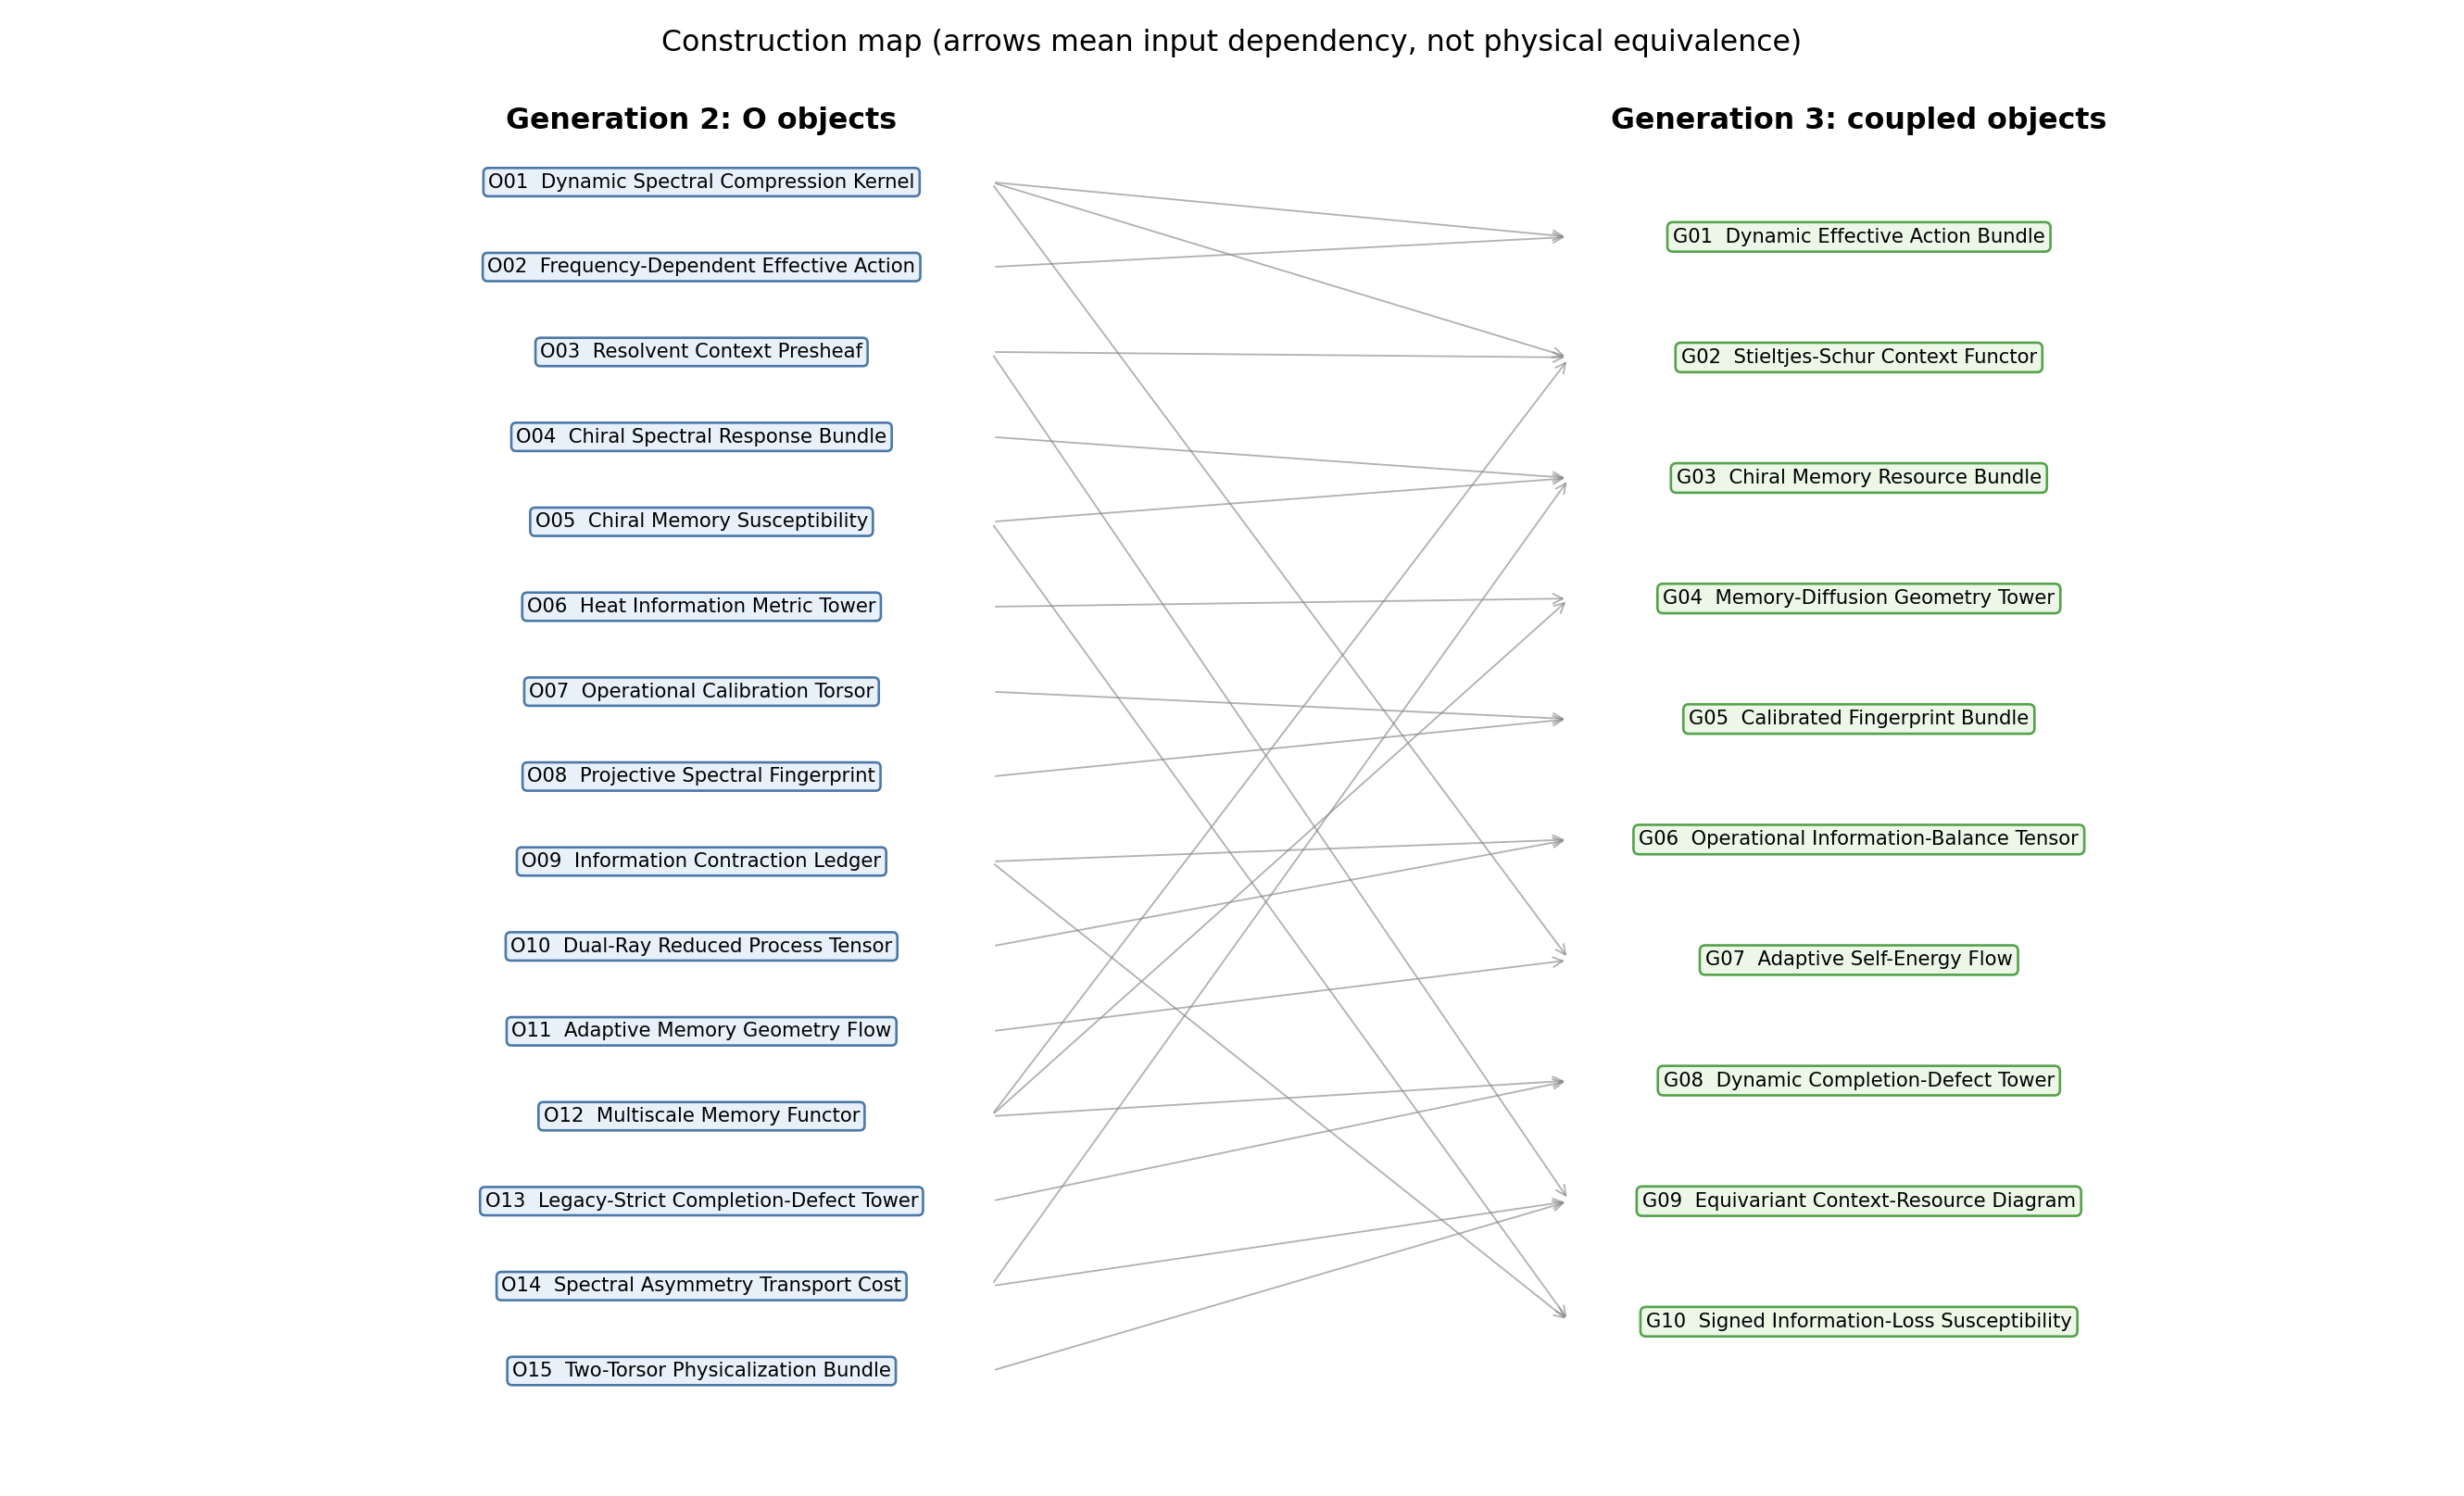
\includegraphics[width=0.97\textwidth]{FIN_Second_Generation_Atlas_Figures/generation2_generation3_map.png}
\caption{Zależności wejściowe między obiektami generacji O i G; strzałki nie oznaczają równoważności fizycznej.}
\end{figure}

\begin{center}
\begingroup\fontsize{7}{8.4}\selectfont
\setlength{\tabcolsep}{2.5pt}
\renewcommand{\arraystretch}{1.16}
\begin{longtable}{@{}p{0.055\textwidth}p{0.160\textwidth}p{0.312\textwidth}p{0.246\textwidth}p{0.087\textwidth}@{}}
\toprule
\textbf{ID} & \textbf{Połączenie} & \textbf{Obiekt wy\.zszego rzędu} & \textbf{Definicja/\allowbreak{}rola} & \textbf{Status} \\
\midrule
\endhead
G01 & O01+O02 & Dynamic Effective Action Bundle & samoenergia Stieltjesa wraz z dokładnym działaniem źródłowym & \statusProven{} \\
G02 & O01+O03+O12 & Stieltjes--Schur Context Functor & funktor kontekstów, zgodne redukcje, całkowicie monotoniczne samoenergie & \statusProven{} \\
G03 & O04+O05+O14 & Chiral Memory Resource Bundle & nieparzysta podatność pamięci z bud\.zetem zasobu asymetrii & \statusStrong{} \\
G04 & O06+O12 & Memory--Diffusion Geometry Tower & geometria indeksowana czasem dyfuzji i głębokością ukrycia & \statusModerate{} \\
G05 & O07+O08 & Calibrated Fingerprint Bundle & bezskalowy test plus jawnie zewnętrzna sekcja skali & \statusProven{} \\
G06 & O09+O10 & Operational Information-Balance Tensor & wieloczasowy ledger kontrakcji informacji & \statusModerate{} \\
G07 & O01+O11 & Adaptive Self-Energy Flow & trajektoria uczona w przestrzeni funkcji Stieltjesa & \statusSpeculative{} \\
G08 & O12+O13 & Dynamic Completion-Defect Tower & test, czy bridge defect przetrwa dynamiczną redukcję & \statusModerate{} \\
G09 & O03+O14+O15 & Equivariant Context-Resource Diagram & konteksty, skala i orientacja jako osobne struktury sekcyjne & \statusSpeculative{} \\
G10 & O05+O09 & Signed Information-Loss Susceptibility & pochodna kontrakcji informacji względem chiralnego skrętu & \statusSpeculative{} \\
\bottomrule
\end{longtable}
\endgroup
\end{center}

\chapter{10. Najwa\.zniejsze "kształty cienia"}

\section{Cień 1 --- brakująca przestrzeń obiektów to Stieltjes space}

Wcześniej pytano, jakie kolejne jądro statyczne otrzymuje się po kompresji. Połączenie Green + Schur + dynamika pokazuje, \.ze właściwym obiektem jest funkcja operatorowa \(z\mapsto\Sigma(z)\).

To zmienia pytanie o samopodobieństwo:

\[
\text{czy }K\text{ jest fixed pointem?}
\]

na:

\[
\text{czy rodzina funkcji pamięci jest zamknięta lub ma atraktor?}
\]

\statusStrong{} jako kierunek; fixed point nie został znaleziony.

\section{Cień 2 --- obserwator i kompresja są dwoma nazwami wyboru kontekstu}

Kompresja wybiera zachowane stopnie swobody. Obserwator wybiera dostępne obserwable. Wspólnym cieniem jest kontekst \(E\) oraz jego operator efektywny \(B_E(z)\).

\statusModerate{} To nie dowodzi, \.ze obserwacja fizyczna jest tylko Schurem; instrument i rekord nadal są wymagane.

\section{Cień 3 --- "ujemna informacja" jest często przepływem do niewidocznego sektora}

Ledger O09 i pamięć O01 sugerują:

\[
\text{spadek dostępnej rozró\.znialności}
\quad\leftrightarrow\quad
\text{korelacje/wycieczki w sektorze }H.
\]

W pełnym, odwracalnym opisie informacja mo\.ze nie znikać; znika z wybranego rekordu. \statusStrong{}

\section{Cień 4 --- chiralność jest tangentem, nie punktem}

\(\Xi_E(z)\) pokazuje, \.ze orientacja mo\.ze objawiać się jako kierunek w przestrzeni operatorów pamięci:

\[
\Xi_E\in T_{\Sigma_E}\operatorname{Stieltjes}_+(E).
\]

To nowa charakterystyka pochodna. Nie wybiera ona, czy tangent ma znak \(+\) czy \(-\). \statusStrong{}

\section{Cień 5 --- fizyczność wymaga dwóch sekcji i jednego procesu}

Najmniejszy cień brakującej fizyki ma trzy niezale\.zne elementy:

\begin{enumerate}
\item 
sekcja skali;

\item 
sekcja orientacji/\allowbreak{}sektora;

\item 
proces operacyjny z przygotowaniem, instrumentem i rekordem.

\end{enumerate}

\.Zaden z trzech nie zastępuje pozostałych. \statusProven{} jako rozdzielenie typów.

\section{Cień 6 --- adaptacja mo\.ze działać na pamięci, nie bezpośrednio na kernelu}

Zamiast:

\[
\dot K=-\nabla_K\mathcal L,
\]

naturalniejszym obiektem mo\.ze być:

\[
\partial_t\Sigma(z;t)
=-\operatorname{grad}_{\Sigma}\mathcal L_{\rm process}.
\]

\statusSpeculative{} Ta zmiana mo\.ze ograniczyć prawo uczenia przez dodatniość i całkowitą monotoniczność.

\section{Cień 7 --- bridge defect mo\.ze być dynamiczny}

Legacy i strict mogą ró\.znić się nie tylko profilem \(d\), lecz strukturą ukrytej pamięci. Test O13/\allowbreak{}G08 mo\.ze wykazać:

\begin{itemize}
\item 
residual zanikający pod redukcją;

\item 
residual stały;

\item 
residual rosnący;

\item 
niezgodność klasy Stieltjesa.

\end{itemize}

\.Zaden z tych wyników nie jest z góry mostem. To nowy pojedynczy, falsyfikowalny atom.

\chapter{11. Falsyfikacja najwy\.zszych interpretacji}

\section{11.1. Czy G02 jest nową teorią kategorii?}

Nie. \statusRefuted{} jako roszczenie o nową dziedzinę.

Łączność Schura i diagramy kontekstów są znanymi strukturami. Nowość projektu mo\.ze polegać na ich u\.zyciu do uporządkowania FIN, nie na autorstwie samej matematyki.

\section{11.2. Czy O05 rozwiązuje selector?}

Nie. \statusRefuted{}

Rodzina \(A(\theta)\) wymaga parametru \(\theta\). Inwersja wysyła \(\theta\to-\theta\), więc \(\Xi\) ma parę znaków. O05 jest dokładnie nowym receiverem.

\section{11.3. Czy O09 jest entropią fizyczną?}

Nie bez dodatkowych danych. \statusRefuted{}

Do termodynamiki potrzeba co najmniej temperatury, Hamiltonianu, protokołu i pełnego ledgeru aparatu/\allowbreak{}resetu.

\section{11.4. Czy O12 dowodzi fraktalnego fixed pointu?}

Nie. \statusRefuted{}

O12 definiuje właściwą przestrzeń poszukiwania. Istnienie atraktora albo samopodobnej miary operatorowej jest otwarte.

\section{11.5. Czy O11 dowodzi biologicznej natury FIN?}

Nie. \statusRefuted{}

Neural operators, reservoir computing i plastyczność dostarczają analogii mechanizmu adaptacji, lecz brak mapy empirycznej.

\section{11.6. Czy G09 daje globalną sekcję?}

Nie. \statusRefuted{} na bie\.zących artefaktach.

Język sekcji podkreśla istniejący obstruction. Nie usuwa QW-2191 ani skali.

\chapter{12. Programy badań 255--266}

\section{Program 255 --- Formalne twierdzenie Stieltjesa dla wszystkich kontekstów}

Udowodnić w jednej bibliotece:

\begin{itemize}
\item 
dodatniość;

\item 
całkowitą monotoniczność;

\item 
reprezentację miarą operatorową;

\item 
granice \(z\to0^+\) i \(z\to\infty\).

\end{itemize}

\textbf{Prawdopodobieństwo sukcesu:} 0.95.

\section{Program 256 --- Minimalna realizacja samoenergii}

Określić, kiedy dwie ukryte macierze \((A_{HH},A_{HE})\) dają tę samą \(\Sigma_E(z)\). U\.zyć controllability/\allowbreak{}observability i minimal realization theory.

\textbf{Prawdopodobieństwo:} 0.85.

\section{Program 257 --- Formalizacja funktora kontekstów}

Zdefiniować kategorię kontekstów i redukcji, a następnie skompilować łączność Schura w Lean/\allowbreak{}Mathlib albo niezale\.znym algebraicznym core.

\textbf{Prawdopodobieństwo:} 0.80.

\section{Program 258 --- Analityczne twierdzenie o chiralnej podatności pamięci}

Wyprowadzić zamknięty wzór na \(\Xi_E(z)\), jego kowariancję i granice normy. Oddzielić gauge convention od obserwabli flux.

\textbf{Prawdopodobieństwo:} 0.82.

\section{Program 259 --- Dynamiczny RG w przestrzeni Stieltjesa}

Zdefiniować mapę:

\[
\mathcal R:\Sigma^{(n)}\mapsto\Sigma^{(n+1)}
\]

i szukać fixed pointów, cykli oraz no-go dla rodziny strict.

\textbf{Prawdopodobieństwo:} 0.45; wysoka nagroda.

\section{Program 260 --- Wieloczasowy tensor bilansu informacji}

Rozszerzyć O09 na proces:

\[
\mathcal L[\mathcal M_1,\ldots,\mathcal M_r]
\]

i oddzielić kontrakcję systemu, aparatu i ukrytych węzłów.

\textbf{Prawdopodobieństwo:} 0.75.

\section{Program 261 --- Dynamiczny test completion defect}

Przetestować dokładnie jeden nowy atom:

\[
\Delta_\Sigma(z)
=\Sigma_{\rm strict}(z)
-\mathcal C_\Sigma[\Sigma_{\rm legacy}(z)].
\]

Reguła stop: nie dostrajać funkcji completion po zobaczeniu celu.

\textbf{Prawdopodobieństwo konstruktywnego bridge:} 0.30.\\
\textbf{Prawdopodobieństwo wartościowego no-go:} 0.80.

\section{Program 262 --- Calibrated Fingerprint Experiment}

Połączyć O07+O08 z P240--P242:

\begin{itemize}
\item 
najpierw test ilorazów widmowych;

\item 
następnie niezale\.zna kalibracja \(\tau\);

\item 
bez zmiany modelu po unblindingu.

\end{itemize}

\textbf{Prawdopodobieństwo metodologicznego sukcesu:} 0.75.

\section{Program 263 --- Tomografia prądów i pamięci chiralnej}

Mierzyć \(C_d\) dla \(d=1,\ldots,5\) oraz interwencje pośrednie. Testować \(C_\chi\) i \(\Xi_E(z)\) oddzielnie.

\textbf{Prawdopodobieństwo:} 0.70.

\section{Program 264 --- False-positive atlas O01--O10}

Wygenerować losowe i strukturalne Laplasjany. Zmierzyć, ile przechodzi:

\begin{itemize}
\item 
strict fingerprint;

\item 
Stieltjes memory;

\item 
context composition;

\item 
chiral response;

\item 
information ledger.

\end{itemize}

\textbf{Prawdopodobieństwo:} 0.90.

\section{Program 265 --- Identyfikowalność Adaptive Memory Geometry}

Porównać O11 z:

\begin{itemize}
\item 
statycznym operatorem;

\item 
aparatem z pamięcią;

\item 
błędną kalibracją;

\item 
prawdziwą zmianą generatora.

\end{itemize}

Wymaga hold-out i kontrprzykładów nieidentyfikowalnych.

\textbf{Prawdopodobieństwo:} 0.65.

\section{Program 266 --- Benchmark biologiczno-cybernetyczny}

Bez roszczeń ontologicznych sprawdzić:

\begin{itemize}
\item 
fading-memory capacity;

\item 
robustness--plasticity trade-off;

\item 
recovery after perturbation;

\item 
minimal readout dimension.

\end{itemize}

FIN przechodzi analogię tylko wtedy, gdy daje przewidywania inne ni\.z standardowy reservoir o tej samej liczbie stanów.

\textbf{Prawdopodobieństwo rozstrzygającego benchmarku:} 0.72.

\chapter{13. Priorytet strategiczny}

\begin{center}
\begingroup\small
\setlength{\tabcolsep}{2.5pt}
\renewcommand{\arraystretch}{1.16}
\begin{longtable}{@{}p{0.183\textwidth}p{0.257\textwidth}p{0.420\textwidth}@{}}
\toprule
\textbf{Ranga} & \textbf{Program} & \textbf{Powód} \\
\midrule
\endhead
1 & 255 & niemal pewne formalne domknięcie nowej przestrzeni obiektów \\
2 & 256 & rozstrzyga, co mo\.zna wnioskować o ukrytym sektorze \\
3 & 258 & domyka nową charakterystykę chiralnej pamięci bez selector claim \\
4 & 257 & zabezpiecza kategorię kontekstów przed metaforycznym u\.zyciem \\
5 & 264 & mierzy swoistość całego atlasu \\
6 & 260 & łączy informację z pełnym procesem \\
7 & 262 & przenosi wynik do laboratorium \\
8 & 263 & eksperymentalnie rozdziela harmoniczne i pamięć \\
9 & 259 & najwy\.zsza nagroda matematyczna, du\.ze ryzyko \\
10 & 261 & pojedynczy uczciwy atak bridge \\
11 & 265 & sprawdza adaptację i identyfikowalność \\
12 & 266 & kontroluje analogie biologiczne/\allowbreak{}cybernetyczne \\
\bottomrule
\end{longtable}
\endgroup
\end{center}

\chapter{14. Granice zgodne z guardrails}

Raport nie eksportuje:

\begin{itemize}
\item 
niepremisowego strict selector;

\item 
rozładowania QW-2191;

\item 
kanonicznej jednostki długości, czasu, masy, energii lub działania;

\item 
pełnej mapy legacy->strict;

\item 
role transfer dla \(\sin^2\theta_W\), \(\alpha_{\rm EM}\) lub hierarchii grawitacyjnej;

\item 
strict-source prawa adaptacyjnego;

\item 
\(L_{\rm total}\), Modelu Standardowego, GR ani ToE;

\item 
dowodu fizycznego obserwatora, środowiska albo aparatu;

\item 
zewnętrznej walidacji danych.

\end{itemize}

Nadsoliton pozostaje pierwotną informacją w stanie solitonicznym. Konteksty \(E/H\) są podziałami dostępności jego stopni swobody, nie osobną warstwą informacyjną pod nim.

\chapter{15. Werdykt końcowy}

Najwa\.zniejszą pochodną strukturą z kombinacji puzzli nie jest kolejne jądro i nie jest nią nowa stała. Jest nią:

\[
\boxed{
\text{Stieltjes--Schur Context Functor}
}
\]

czyli kontekstowa rodzina dokładnych operatorów efektywnych, których samoenergie są całkowicie monotoniczne, redukcje składają się, a transformacje czasowe generują pamięć.

Ta struktura porządkuje wspólny cień:

\[
\text{Green}
\leftrightarrow
\text{kompresja}
\leftrightarrow
\text{pamięć}
\leftrightarrow
\text{obserwator}
\leftrightarrow
\text{informacja dostępna}.
\]

Najciekawszą nową charakterystyką tangentową jest \(\Xi_E(z)\): chiralna podatność pamięci. Najuczciwszym opisem ubytku informacji jest \(\mathcal L_t\): kontrakcja dostępnej rozró\.znialności. Najwa\.zniejszym no-go pozostaje brak sekcji orientacji i skali.

To nie potwierdza FIN jako fizyki. Dostarcza jednak nowej, ścisłej przestrzeni obiektów, w której następne pytania są lepiej typowane i łatwiejsze do falsyfikacji.

\chapter{16. Literatura porównawcza}

\begin{enumerate}
\item 
Dörfler, F.; Bullo, F., \emph{Kron Reduction of Graphs with Applications to Electrical Networks}, \href{https://arxiv.org/abs/1102.2950}{https:/\allowbreak{}/\allowbreak{}arxiv.org/\allowbreak{}abs/\allowbreak{}1102.2950}.

\item 
Lin, Y. T.; Tian, Y.; Anghel, M.; Livescu, D., \emph{Data-driven learning for the Mori--Zwanzig formalism}, \href{https://arxiv.org/abs/2101.05873}{https:/\allowbreak{}/\allowbreak{}arxiv.org/\allowbreak{}abs/\allowbreak{}2101.05873}.

\item 
Pollock, F. A. et al., \emph{Non-Markovian quantum processes: complete framework and efficient characterisation}, \href{https://arxiv.org/abs/1512.00589}{https:/\allowbreak{}/\allowbreak{}arxiv.org/\allowbreak{}abs/\allowbreak{}1512.00589}.

\item 
Marvian, I.; Spekkens, R. W., \emph{Modes of asymmetry}, \href{https://arxiv.org/abs/1312.0680}{https:/\allowbreak{}/\allowbreak{}arxiv.org/\allowbreak{}abs/\allowbreak{}1312.0680}.

\item 
Coifman, R. R.; Lafon, S., \emph{Diffusion maps}, \href{https://doi.org/10.1016/j.acha.2006.04.006}{https:/\allowbreak{}/\allowbreak{}doi.org/\allowbreak{}10.1016/\allowbreak{}j.acha.2006.04.006}.

\item 
Shuman, D. I. et al., \emph{The Emerging Field of Signal Processing on Graphs}, \href{https://arxiv.org/abs/1211.0053}{https:/\allowbreak{}/\allowbreak{}arxiv.org/\allowbreak{}abs/\allowbreak{}1211.0053}.

\item 
Kovachki, N. et al., \emph{Neural Operator: Learning Maps Between Function Spaces}, \href{https://arxiv.org/abs/2108.08481}{https:/\allowbreak{}/\allowbreak{}arxiv.org/\allowbreak{}abs/\allowbreak{}2108.08481}.

\item 
Abramsky, S.; Brandenburger, A., \emph{The Sheaf-Theoretic Structure of Non-Locality and Contextuality}, \href{https://arxiv.org/abs/1102.0264}{https:/\allowbreak{}/\allowbreak{}arxiv.org/\allowbreak{}abs/\allowbreak{}1102.0264}.

\item 
Chamseddine, A. H.; Connes, A., \emph{The Spectral Action Principle}, \href{https://arxiv.org/abs/hep-th/9606001}{https:/\allowbreak{}/\allowbreak{}arxiv.org/\allowbreak{}abs/\allowbreak{}hep-th/\allowbreak{}9606001}.

\end{enumerate}

\chapter{17. Artefakty reprodukowalne}

\begin{itemize}
\item 
fin\_nadsoliton\_second\_generation\_atlas.py

\item 
FIN\_Second\_Generation\_Combination\_Search.csv

\item 
FIN\_Second\_Generation\_Derived\_Objects.csv

\item 
FIN\_Second\_Generation\_Generation3.csv

\item 
FIN\_Second\_Generation\_Atlas\_Results.json

\item 
FIN\_Second\_Generation\_Atlas\_Figures/\allowbreak{}combination\_search\_coverage.png

\item 
FIN\_Second\_Generation\_Atlas\_Figures/\allowbreak{}derived\_object\_score\_matrix.png

\item 
FIN\_Second\_Generation\_Atlas\_Figures/\allowbreak{}generation2\_generation3\_map.png

\item 
FIN\_Atlas\_Drugiej\_Generacji\_Pochodne\_Obiekty\_Nadsolitona\_PL.md

\end{itemize}


\clearpage
\chapter*{Reprodukcja}
\addcontentsline{toc}{chapter}{Reprodukcja}
\begin{Verbatim}[fontsize=\small]
MPLCONFIGDIR=/tmp/matplotlib-second \
python3 fin_nadsoliton_second_generation_atlas.py
\end{Verbatim}
Oczekiwane pokrycie: 305 kombinacji, 15 obiektów generacji O i 10 obiektów
generacji G.  Gramatyka konstrukcji jest filtrem kandydatów, nie dowodem
równoważności ani fizyczności.
\end{document}
